\documentclass[t]{beamer}

%\documentclass[handout, t]{beamer}
\setbeamertemplate{navigation symbols}{}

 
\usepackage{amsfonts}
\usepackage{mathrsfs}
\usepackage{amsmath}
\usepackage{multicol}

\usepackage{bm}
\usepackage[UTF8]{ctex}
\usetheme{AnnArbor}
\usefonttheme{serif}
\useinnertheme{rounded}
%\usecolortheme{crane}
\setbeamertemplate{blocks}[rounded][shadow=true]

\usepackage{graphicx}

\setmainfont{Times New Roman}
\setCJKmainfont{Microsoft YaHei}
\usepackage{tikz}
\usetikzlibrary{arrows, decorations.pathmorphing, backgrounds, positioning, fit, petri, automata}
\tikzset{>=stealth}

\hypersetup{pdfpagemode=FullScreen}
\renewcommand{\Pr}{\mathbb{P}}
\newcommand{\E}{\mathbb{E}}

\usepackage{blkarray}


\setbeamercolor{block title}{bg=red!10!white}
\setbeamercolor{block body}{bg=gray!5!white}

\newcommand{\dif}{{\;\rm d}}

\usepackage{listings}


\lstset{
  language=Python, % 设置语言
  basicstyle=\ttfamily, % 设置字体族
  breaklines=true, % 自动换行
  keywordstyle=\bfseries\color{blue}, % 设置关键字
  ndkeywordstyle=\bfseries\color{blue}, % 设置关键字
  classoffset=0,
  emph=[0]{self, plt, pd, np, print, sm, sns, None, True, False}, % 指定强调词,如果有多个,用逗号隔开
  emphstyle=\bfseries\color{magenta!90!black}, % 强调词样式设置
  classoffset=1,
  moreemph=[1]{plot, text, title, show, scatter, as, figure, xlabel, ylabel, fit, mean}, % 设置更多的关键字,用逗号分隔
  emphstyle=\bfseries\color{blue}, % 强调词样式设置
  classoffset=0,
  commentstyle=\itshape\color{gray}, % 设置注释样式,斜体,浅灰色
  stringstyle=\bfseries\color{green!50!black}, % 设置字符串样式
  columns=flexible,
  numberstyle=\footnotesize, % 缩小行号
}

\begin{document}
\fontsize{11}{18}\selectfont


\CTEXindent


\title{第一章~~自动化数据采集及清洗1}

\author{主讲:方杰、李烜}
\date{福建江夏学院金融学院}

\maketitle

\begin{frame}{本章目录}
      \tableofcontents  
\end{frame}


\section{应用程序接口}

\begin{frame}{应用程序接口}
 
应用程序接口(API,Application Programming Interface)是一个{\color{red}预定义的函数},这个函数中约定了数
据资源提供方的通信规则。通过应用程序接口可以实现相
互独立的系统之间的数据请求、获取和调用。

\begin{block}{工作机制}
    资源提供方提供标准接
口文档$\longrightarrow$调用方按需选
择接口并传入相关参数
$\longrightarrow $资源提供方服务器接
收请求,进行业务处理,
返回数据。
\end{block}


\end{frame}


\begin{frame}{API的优点}
\begin{itemize}
    \item 简单、易用
    \item 能设置报错机制,便于监控
    接口运行情,及时排除故障
    \item 分页和过滤功能节省服务器
    资源和带宽,以支持企业级
    的高并发和大容量
    \item 设置访问权限,提高信息的
    安全性
    \item 可平滑的移植和扩展,以保
    证系统的稳定性
\end{itemize}
\end{frame}




\begin{frame}{API的缺点}
\begin{itemize}
    \item 需要用不同的语言封
    装,增加了设计复杂
    度
    \item 封装后降低代码的可
    复用性,也可能会降
    低程序的执行效率
\end{itemize}


\end{frame}

\section{Python模块和包的概念}
\subsection{Python模块}

\begin{frame}{Python模块}
    Python 模块(Module),本质上是一个Python程序,以.py作为文件后缀,任何py文件都可以作为一个模块。模块能定义函数、类和变量,也能包含可执行的代码。
    
    Python模块一共有三种:
\begin{enumerate}
    \item Python内置模块(标准库)
    \item 第三方模块
    \item 应用程序/自定义的模块
\end{enumerate}
\end{frame}

\begin{frame}[fragile]{简单的Python模块\texttt{module1.py}}
\begin{lstlisting}
# 定义一个打印函数
def print_func(par):
    print('Hello:', par)
    return

# 定义一个求和函数
def sum(x,y):
    print('sum:', x+y)
    return x+y
\end{lstlisting}


\end{frame}

\subsection{Python包}
\begin{frame}[fragile]{Python包}
    Python按目录来组织模块,称为包(Package)。

    包类似文件夹,用来管理和
    分类模块的。这个文件夹下
    必须存在\verb|__init__.py| 文件,
    用于标识当前文件夹是一个
    包。    

包是一个分层次的文件
目录结构,定义了一个
由模块、子包、子包下
的子包等组成的
Python 的应用环境。

\begin{block}{演示:}
    Python包\texttt{Numpy}中的文件及目录结构。
\end{block}
\end{frame}


\begin{frame}[fragile]{Python包举例}
    在\verb|package_run|目录下,创建
    \verb|runtest1.py|、\verb|runtest2.py|、\verb|__init__.py|三个文件。

    \small
\begin{multicols}{2}
    \centering  {\color{red}\verb|runtest1.py|}
\begin{lstlisting}
def test1():
    print('I am in runtest1')
def sum1(x,y):
    print('sum1:',x+y)
    return x+y
\end{lstlisting}

{\color{blue}
\verb|runtest2.py|}
\begin{lstlisting}
def test2():
    print('I am in runtest2')
def sum2(x,y):
    print('sum2:',x+y)
    return x+y
\end{lstlisting}
\end{multicols}

\centering  {\color{cyan}\verb|__init__.py|}
\begin{lstlisting}
    __all__=['runtest2']  #定义加载子模块的名称是runtest2
\end{lstlisting}

\end{frame}



\begin{frame}[fragile]{包导入与函数引用:\texttt{import}}
    对于已定义的包,可以使用\texttt{import}语句来导入包
\begin{lstlisting}
    import 包名称
\end{lstlisting}
该方法导入包中\verb|__init__.py|文件所定义的模块

\begin{lstlisting}
# 导入自定义Python 包package_run
import package_run              #导入包
package_run.runtest2.test2()   
            #调用runtest2.py中的函数test2
\end{lstlisting}

\begin{block}{注意:}
此时无法调用\verb|runtest1.py|中的函数
\end{block}
\end{frame}


\begin{frame}[fragile]{包导入与函数引用:\texttt{from ... import ...}}
    使用\texttt{from ... import ...}语句,可以从包中导入指定的模块
\begin{lstlisting}
    from 包名称 import 模块名称
\end{lstlisting}

导入包\verb|package_run| 下的\verb|runtest1|模块
\begin{lstlisting}  
from package_run import runtest1   #导入包中的模块
runtest1.test1()     #调用runtest1模块中的函数test1
\end{lstlisting}

\end{frame}


\begin{frame}[fragile]{包导入与函数引用:\texttt{from ... import *}}
使用\texttt{from ... import *}语句导入包中\verb|__init__.py|文件所定义的模块,具体语法为:
\begin{lstlisting}
from 包名称 import *
模块名.函数名
\end{lstlisting}

导入\verb|package_run|包中的\verb|runtest2|模块,并调用其中的\verb|test2|函数
\begin{lstlisting}
from package_run import *     #导入包中的所有模块
runtest2.test2()       #调用runtest2模块中的test2函数
\end{lstlisting}

\end{frame}

\begin{frame}[fragile]{举例:}
\begin{block}{输出$\sqrt{2}$的结果}
\begin{multicols*}{2}
    \centering
    方法1:
    \begin{lstlisting}
import math
print(math.sqrt(2))
\end{lstlisting}
方法2:
\begin{lstlisting}
from math import *
print(sqrt(2))
\end{lstlisting}
\end{multicols*}    
\end{block}



\begin{block}{输出$\pi$的结果}
\begin{lstlisting}
from math import pi
print(pi)      
\end{lstlisting}    
\end{block}
\end{frame}



\begin{frame}{API接口调用的Python包}
\begin{itemize}
    \item \texttt{requests}
    \item \texttt{pandas}
    \item \texttt{numpy}
    \item \texttt{matplotlib}
    \item \texttt{OnePlusX}
    \item …………
\end{itemize}
\end{frame}

\begin{frame}[fragile]{\texttt{requests}}
    \texttt{requests}专门用于发送HTTP请求,\texttt{requests}包中最常用的是\texttt{get}和\texttt{post}请求函数。

\begin{block}{\texttt{get}函数}
    \texttt{get}函数用于向服务器请求传送数据
\begin{lstlisting}
    requests.get(url)
\end{lstlisting}
\end{block}

\begin{block}{\texttt{post}函数}
    \texttt{post}函数向服务器传送数据,并且可以携带请求参数
\begin{lstlisting}
    requests.post(url,data=None,json=None)
\end{lstlisting}
\end{block}
\end{frame}

\begin{frame}[fragile]{\texttt{post}函数}
    \begin{lstlisting}
        requests.post(url, data=None, json=None)
    \end{lstlisting}
\begin{itemize}
    \item 参数\verb|url|是拟获取页面的网址,{\color{red}不可省略}
    \item 参数\verb|data|是指定的获取条件,可省略
    \item 参数\verb|json|表示请求是以\verb|json|形式发送请求
\end{itemize}

\begin{block}{\texttt{json}是什么?}
    JSON(JavaScript Object Notation)是一种轻量级的数据交换格式。易于阅读和编写,可以在多种语言之间进行数据交换。
\end{block}
\end{frame}

\begin{frame}[fragile]{例:获取某平台上张三的信息}
\begin{lstlisting}
import requests            # 导入包
targetUrl = 'http://www.iyyyf.com'      # 服务器地址
data = {'name':'张三',  'age':20}
# 向请求地址并传递data参数
response = requests.post(targetUrl, data = data) 
\end{lstlisting}
\end{frame}

\begin{frame}[fragile]{\texttt{pandas}包}
    \texttt{pandas}包可将接口调取的数据输出到excel文件中
\begin{lstlisting}
df.to_excel(文件位置及名称, sheet_name=0, columns=None, 
            header=True, usecols=None, dtype=None)
\end{lstlisting}

\begin{block}{例:将获取到的price数据存储为excel文档}
\begin{lstlisting}
    price.to_excel('D:\price_data.xlsx')
\end{lstlisting}
\end{block}

\begin{block}{其他类似的命令}
\begin{lstlisting}
df.to_csv(),   df.to_sql(),   df.to_hdf()
\end{lstlisting}    
\end{block}
\end{frame}

\begin{frame}{\texttt{OnePlusX}包}
    \texttt{OnePlusX}包是数
据资源方CSMAR数据公司所
定义的数据接口服务包,包
中封装了\texttt{OnePlusXService}
类。其中的\texttt{OnePlusXClass}模块中包含了许多接口调用函数
\begin{itemize}
    \item 查看数据表\texttt{getTableList()}
    \item 查看表格字段\texttt{getListFields}
    \item 预览数据\texttt{preview}
    \item 条件查询\texttt{query}
\end{itemize}
\end{frame}

\begin{frame}{\texttt{OnePlusX}包的层次关系}
    \centering
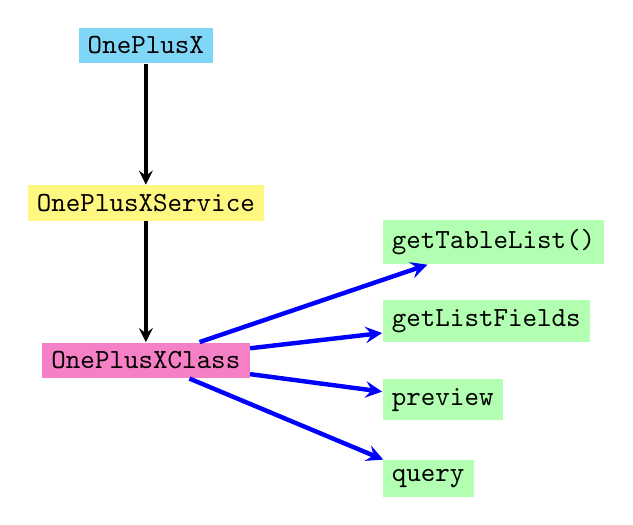
\begin{tikzpicture}
    \node[fill=cyan!50!white] (A) at (0,0) {\texttt{OnePlusX}};
\node[fill=yellow!50!white] (B) at (0,-2) {\texttt{OnePlusXService}};
\node[fill=magenta!50!white] (C) at (0,-4) {\texttt{OnePlusXClass}};
\draw[->, very thick](A)--(B);
\draw[->, very thick](B)--(C);

\node[fill=green!30!white, right] (D1) at (3,-2.5) {\texttt{getTableList()}};
\node[fill=green!30!white, right] (D2) at (3,-3.5) {\texttt{getListFields}};
\node[fill=green!30!white, right] (D3) at (3,-4.5) {\texttt{preview}};
\node[fill=green!30!white, right] (D4) at (3,-5.5) {\texttt{query}};
\draw[->, ultra thick, blue](C)--(D1);
\draw[->, ultra thick, blue](C)--(D2);
\draw[->, ultra thick, blue](C)--(D3);
\draw[->, ultra thick, blue](C)--(D4);

\end{tikzpicture}


\end{frame}



\begin{frame}{任务实施(见P21)}
两种方法:
\begin{enumerate}
    \item 调用API,基于\texttt{OnePlusX}包进行数据的调用及处理
    \item 使用\texttt{requests}包,通过Web Service API进行调用
\end{enumerate}

\vskip 1cm

三个步骤:
\begin{enumerate}
    \item 查询数据表
    \item 查看数据表的字段(field)列表
    \item 根据条件查询数据
\end{enumerate}
\end{frame}

\section{结构化数据处理}


\begin{frame}[fragile]{结构化数据}
结构化数据,是指可以使用二维表结构表示和存储的数据,具有易于输入、存储、查询和分析的特点。

使用Python对表结构 的数据 进行处理,需要掌握\verb|Pandas|库的DataFrame数据结构。

\end{frame}


\subsection{DataFrame数据结构}
\begin{frame}[fragile]{DataFrame(数据帧)}
    使用DataFrame首先需要导入\verb|Pandas|包,Pandas({\color{red}Pan}el {\color{red}d}ata {\color{red}a}nalysi{\color{red}s})是Python的一个数据
    分析包,内含大量库和一些标准的数据模型。

    DataFrame是\verb|Pandas|中一种表格型数据结构,是结构化数据在
    Python语言中的一种表现形式。

    构建DataFrame对象的方法:
\begin{enumerate}
    \item 从字典构造
    \item 从表格文件(excel, csv,...)构造
\end{enumerate}

\end{frame}


\begin{frame}[fragile]{什么是字典(dict)?}
    字典是Python内存放具有映射关系的表结构数据的常用方式。
字典中的内容放在$\{\ldots\}$里,其中保存了一一对应的若干组数据,以“键 : 值”的方式存储。

\begin{lstlisting}
{key1 : value1, key2 : value2, key3 : value3, ....}
\end{lstlisting}


键(key)是关键字,相当于数据库中的字段(field),{\color{red}键是不能重复的};值(value)是键所对应的值,相当于数据库中的记录(record)。

\begin{block}{注意:}
    \texttt{json}文件具有类似于字典的数据结构。通常可以利用json文件的文本,生成字典。
\end{block}

\end{frame}


\begin{frame}[fragile]{字典方式构建DataFrame对象}
    构建DataFrame对象时,先定义数据字典,再将字典转化为DataFrame对象。

\begin{block}{构造方式}
   \begin{lstlisting}
import pandas as pd
data = { 列名称A : [数据A1, 数据A2, ...],
         列名称B : [数据B1, 数据B2, ...], ...}
df = pd.DataFrame(data)
\end{lstlisting} 
\end{block}    

\begin{block}{注意:}
此时DataFrame的{\color{red}行索引}是从0开始的整数。我们可以通过\texttt{\color{red}index}选项对行索引进行修改。\texttt{\color{blue}columns}选项则可以修改{\color{blue}列索引}的名称。
\end{block}
\end{frame}


\begin{frame}[fragile]{从表格文件构建DataFrame对象}
对于已存在的表格文件,可以使用\verb|Pandas|将其中的数据转换为DataFrame对象。

\begin{lstlisting}
    import pandas as pd
    df1 = pd.read_excel(r'D:\abc\test.xlsx', 
                            sheet_name=Sheet2)
    df2 = pd.read_csv(r'D:\abc\test.csv')
\end{lstlisting}
\begin{block}{提示:}
若csv文件中有非西文字符(如汉字),务必确保文件的编码是{\color{red}UTF-8},否则表格的读取会报错
\end{block}
\end{frame}

\begin{frame}{DataFrame中数据的提取}
常用的方式:
\begin{enumerate}
    \item \texttt{df[columns][index]}:获取df中{\color{blue}行索引值}为index,{\color{blue}列索引值}为columns的数据(先列后行)
    \item \texttt{df.loc[index, columns]}:结果同上(先行后列)
    \item \texttt{df.iloc[val1,val2]}:获取df中{\color{red}行索引位置}为val1,{\color{red}列索引位置}为val2的数据,只接受从0开始的{\color{red}整数}(integer)
\end{enumerate}

\begin{block}{说明:}
\begin{itemize}
    \item \texttt{loc}: {\color{blue}loc}ation
    \item \texttt{iloc}: {\color{red}i}nteger {\color{red}loc}ation
\end{itemize}
\end{block}
\end{frame}

\begin{frame}[fragile]{获取DataFrame的某一列数据}
获取DataFrame对象\verb|df|中所有基金简称列的数据
\begin{lstlisting}
    print(df['基金简称'])
    print(df.loc[:, '基金简称'])
    print(df.iloc[:, 0])
\end{lstlisting}
\begin{block}{说明:}
    “基金简称”这一列在\verb|df|中位于第一列,因此列索引位置的序号为0
\end{block}
\end{frame}


\begin{frame}[fragile]{获取DataFrame的多列数据}
    获取DataFrame对象\verb|df|中所有基金简称和基金代码数据
\begin{lstlisting}
    print(df[['基金简称', '基金代码']]) 
    print(df.loc[:, ['基金简称','基金代码']])
    print(df.iloc[:, [0,2]])
\end{lstlisting}
\begin{block}{说明:}
    多个列名需要存入列表(list)\verb|[ ]|来表示。“基金简称”和“基金代码”在\verb|df|中位于第1列和第3列,因此列索引位置的序号分别为0和2
\end{block}

\end{frame}

\begin{frame}[fragile]{获取DataFrame的某一行数据}
    获取上文DataFrame对象\verb|df|中第2行的数据
\begin{lstlisting}
    print(df.loc['二']) # 第2行的行索引值为“二”
    print(df.iloc[1])
\end{lstlisting}

\begin{block}{说明:}
    Python中位置序号从0开始,因此第2行在序列位置中记为1
\end{block}
\end{frame}


\begin{frame}[fragile]{获取DataFrame的多行数据}
    获取DataFrame对象\verb|df|中第2、3行的数据
\begin{lstlisting}
    print(df.loc[['二', '三']]) 
    print(df.iloc[[1, 2]])
\end{lstlisting}

\begin{block}{注意:}
多个行名时需要存入列表(list)\verb|[ ]|来表示;第2、3行的位置分别记为1、2。
\end{block}
\end{frame}


\subsection{数据的读写}
\begin{frame}[fragile]{数据的读写}
可以通过Pandas提供的多种读写函数将表格型数据读取为DataFrame对象。
\begin{multicols*}{2}
    \begin{itemize} 
    \item \verb|pd.read_excel|
    \item \verb|pd.to_excel|
    \item \verb|pd.read_csv|
    \item \verb|pd.to_csv|
    \item \verb|pd.read_json|
    \item \verb|pd.to_json|
    \item \verb|read_table|
\end{itemize}
\end{multicols*}

\end{frame}


\begin{frame}[fragile]{从Excel文件读取数据}
\begin{itemize}
    \item 确定文件在系统中所存放的路径。本任务的操作全部基于
    Windows操作系统,在电脑中找到文件,鼠标右键查看文件
    属性,即可得到文件路径。
    \item 将位置和文件名进行组合,得到文件的完整路径。
    其中位置与文件名之间要用目录分隔符隔开(用\verb|/|或者\verb|\\|)。
    \item 使用Pandas中的\verb|pd.read_excel()|函数,将文件路径作为参数,将Excel文件中的数据读入并转化为DataFrame对象形
    式。
\end{itemize}
\end{frame}

\begin{frame}[fragile]{\texttt{pd.read\_excel()}函数的使用方法}
\begin{lstlisting}
pd.read_excel(io, sheet_name=0, header=0, names=None, 
             index_col=None, usecols=None, dtype=None)
\end{lstlisting}
\begin{itemize}
    \item \verb|io| 读取文件的路径,URL地址等
    \item \verb|sheet_name| 需要读取的Excel文件中sheet页的名字
    \item  \verb|header| 指定哪一行做为列索引
    \item  \verb|names| 设置列索引,默认不指定
    \item   \verb|index_col| 指定哪一列做为行索引,默认不指定,自动从0开始生成索引号
    \item  \verb|usecols| 指定读取的列,默认全部读取
    \item  \verb|dtype| 指定读取列数据的数据类型(data type)
\end{itemize}


\end{frame}


\begin{frame}[fragile]{将数据写入Excel文件}
    当数据经过预处理之后,如需将清洗后的数据存写入Excel文件中,可使用\verb|to_excel()|函数
\begin{lstlisting}
df.to_excel(excel_writer, sheet_name=0, columns=None,
             header=True, index=True)
\end{lstlisting}
\begin{itemize}
    \item  \verb|excel_writer| 写入的路径对象。
    \item  \verb|sheet_name| 将数据写入的Excel文件某个指定的sheet中。
    \item  \verb|columns| 需要写入文件的列索引,默认所有列都写入文件。
    \item   \verb|header| 是否将列索引写入文件,默认写入列名。
    \item  \verb|index| 是否将行索引写入文件,默认写入行索引。
\end{itemize}
\end{frame}

\begin{frame}[fragile]{从CSV文件读取数据}
CSV(Comma-Separated Value, 逗号分隔值)文件以纯文本形式存储表格数据(数字和文本),每条记录由字段组成,字段间通常以逗
号或制表符(Tab, \verb|\t|)隔开,每条记录间以换行符分隔。

Pandas中以\verb|pd.read_csv()|函数将CSV文件数据读入
\end{frame}


\begin{frame}[fragile]{\texttt{pd.read\_csv()}函数的使用方法}
\begin{lstlisting}
pd.read_csv(filepath, sep=',', header='infer', names=None, 
         index_col=None, usecols=None, skip_blank_lines=True)   
\end{lstlisting}
\begin{itemize}
    \item \verb|filepath| 读取文件的路径,URL链接等
    \item \verb|sep| 指定CSV文件中的分隔符,默认用逗号分隔,可以指定\verb|\n|(换行符)、\verb|\r|(回车符)、\verb|\t|(制表符)等
    \item \verb|header| 指定某行作为列索引
    \item  \verb|names| 设置列索引,默认不指定
    \item \verb|index_col| 指定哪一列作为Dataframe的行索引,默认没有列索引,自动添加0、1、2....
    \item  \verb|usecols| 指定读取CSV文件的某些列
    \item  \verb|skip_blank_lines| 是否跳过空白行,默认不读空白行
\end{itemize}
\end{frame}


\begin{frame}[fragile]{将数据写入CSV文件}
    当需要把新的数据写入CSV文件进行保存时使用\verb|to_csv()|函数
\begin{lstlisting}
df.to_csv(path_or_buf, sep=',', na_rep='', 
           columns=None, header=True, index=True)
\end{lstlisting}
\begin{itemize}
    \item \verb|path_or_buf| 输出文件路径或者文件对象
    \item \verb|sep| 同一行记录中,各字段间的分隔符,默认为逗号
    \item \verb|na_rep| 空值的替代字符,默认为空字符串
    \item \verb|columns| 要写入文件中的\verb|df|中的列,默认为全部列
    \item \verb|header| 是否将列索引写入文件,默认写入列索引
    \item \verb|index| 是否将行索引写入文件,默认写入行索引
\end{itemize}
\end{frame}

\end{document}